\section{Quelltext und Bilder}

Das Einbinden von Quelltexten ist in \LaTeX mit dem Listings-Paket sehr komfortabel m�glich. Es lassen sich verschiedene Sprachen definieren und man kann aktiv in die Darstellung der einzelnen Sprachelemente eingreifen.

%************** XML ******************
\subsection{XML}
Beispiel f�r XML-Code siehe Quelltext \ref{lst_xml_code}

\lstinputlisting[caption=Beispiel f�r XML-Code, label=lst_xml_code, style=xml]{content/listings/xml_code.xml}


%************** JAVA ******************
\subsection{JAVA}
Beispiel f�r Java-Code siehe Quelltext \ref{lst_java_code}

\lstinputlisting[caption=Beispiel f�r Java-Code, label=lst_java_code, style=java]{content/listings/java_code.java}


%************** BILDER ******************
\subsection{Bilder}
Beispiel um ein Bild einzuf�gen siehe Abbildung \ref{fig:FB4Bild}

\begin{figure}[htb]
	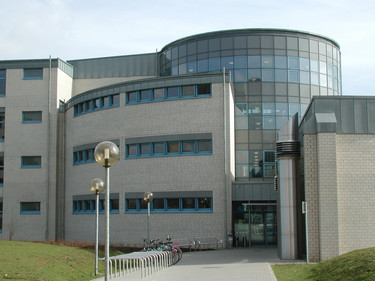
\includegraphics{content/images/52_Foto_FHDortmund_Gebaeude.jpg}
	\caption{Geb�ude des FB4}
	\label{fig:FB4Bild}
\end{figure}


%************** FORMELN ******************
\subsection{Formeln}
Einfache Formeln oder einzelne mathematische Symbole k�nnen durch das Dollar-Zeichen \$ eingebunden werden: \$ Formel \$. Eine so erstellte Formel k�nnte folgenderma�en aussehen:
\begin{center}
	$X(z) = \sum_{n=-\infty}^\infty ( x[n]  * r^{-n} ) * e^{-j\omega n}$ \\
\end{center}

Werden in dem Dokument viele Formeln verwendet und soll bei Bedarf noch einmal darauf zur�ckgegriffen werden k�nnen, macht es Sinn Formeln zu nummerieren. Dazu m�ssen Formeln folgenderma�en eingebunden werden:\\

\textbackslash begin\{equation\textbraceright \\
	\noindent\hspace*{10mm} Hier die Formel\\
\textbackslash end\{equation\textbraceright

Das Ergebnis k�nnte so aussehen:
\begin{equation}
		t-t_{0}=\sqrt{\frac{l}{g}}\int_{0}^{\varphi}{\frac{d\psi}{\sqrt{1-k^{2}\sin^{2} {\psi}}}} = \sqrt{\frac{l}{g}} F(k,\varphi)
\end{equation}